\documentclass[tikz,border=2pt]{standalone}
\usetikzlibrary{positioning}
\usepackage{amsmath, amssymb}
\usepackage{cancel}

\usepackage{anyfontsize} % allows arbitrary font sizes
\usepackage{lmodern} % better font scaling

\makeatletter
\renewcommand\small{%
  \@setfontsize\small{14pt}{16pt}%
}
\renewcommand\normalsize{%
  \@setfontsize\normalsize{16pt}{19pt}%
}
\renewcommand\Large{%
  \@setfontsize\Large{20pt}{24pt}%
}
\makeatother

% Red cancel line but black text
\newcommand{\redcancel}[1]{%
  \tikz[baseline=(X.base)]{
    \node[inner sep=0pt] (X) {$#1$};
    \draw[red,line width=1pt] (X.south west) -- (X.north east);
  }%
}

% Cross.
\newcommand{\Cross}{$\mathbin{\tikz [solid,x=2ex,y=2ex,line width=.4ex, red] \draw (0,0) -- (1,1) (0,1) -- (1,0);}$}%

\begin{document}

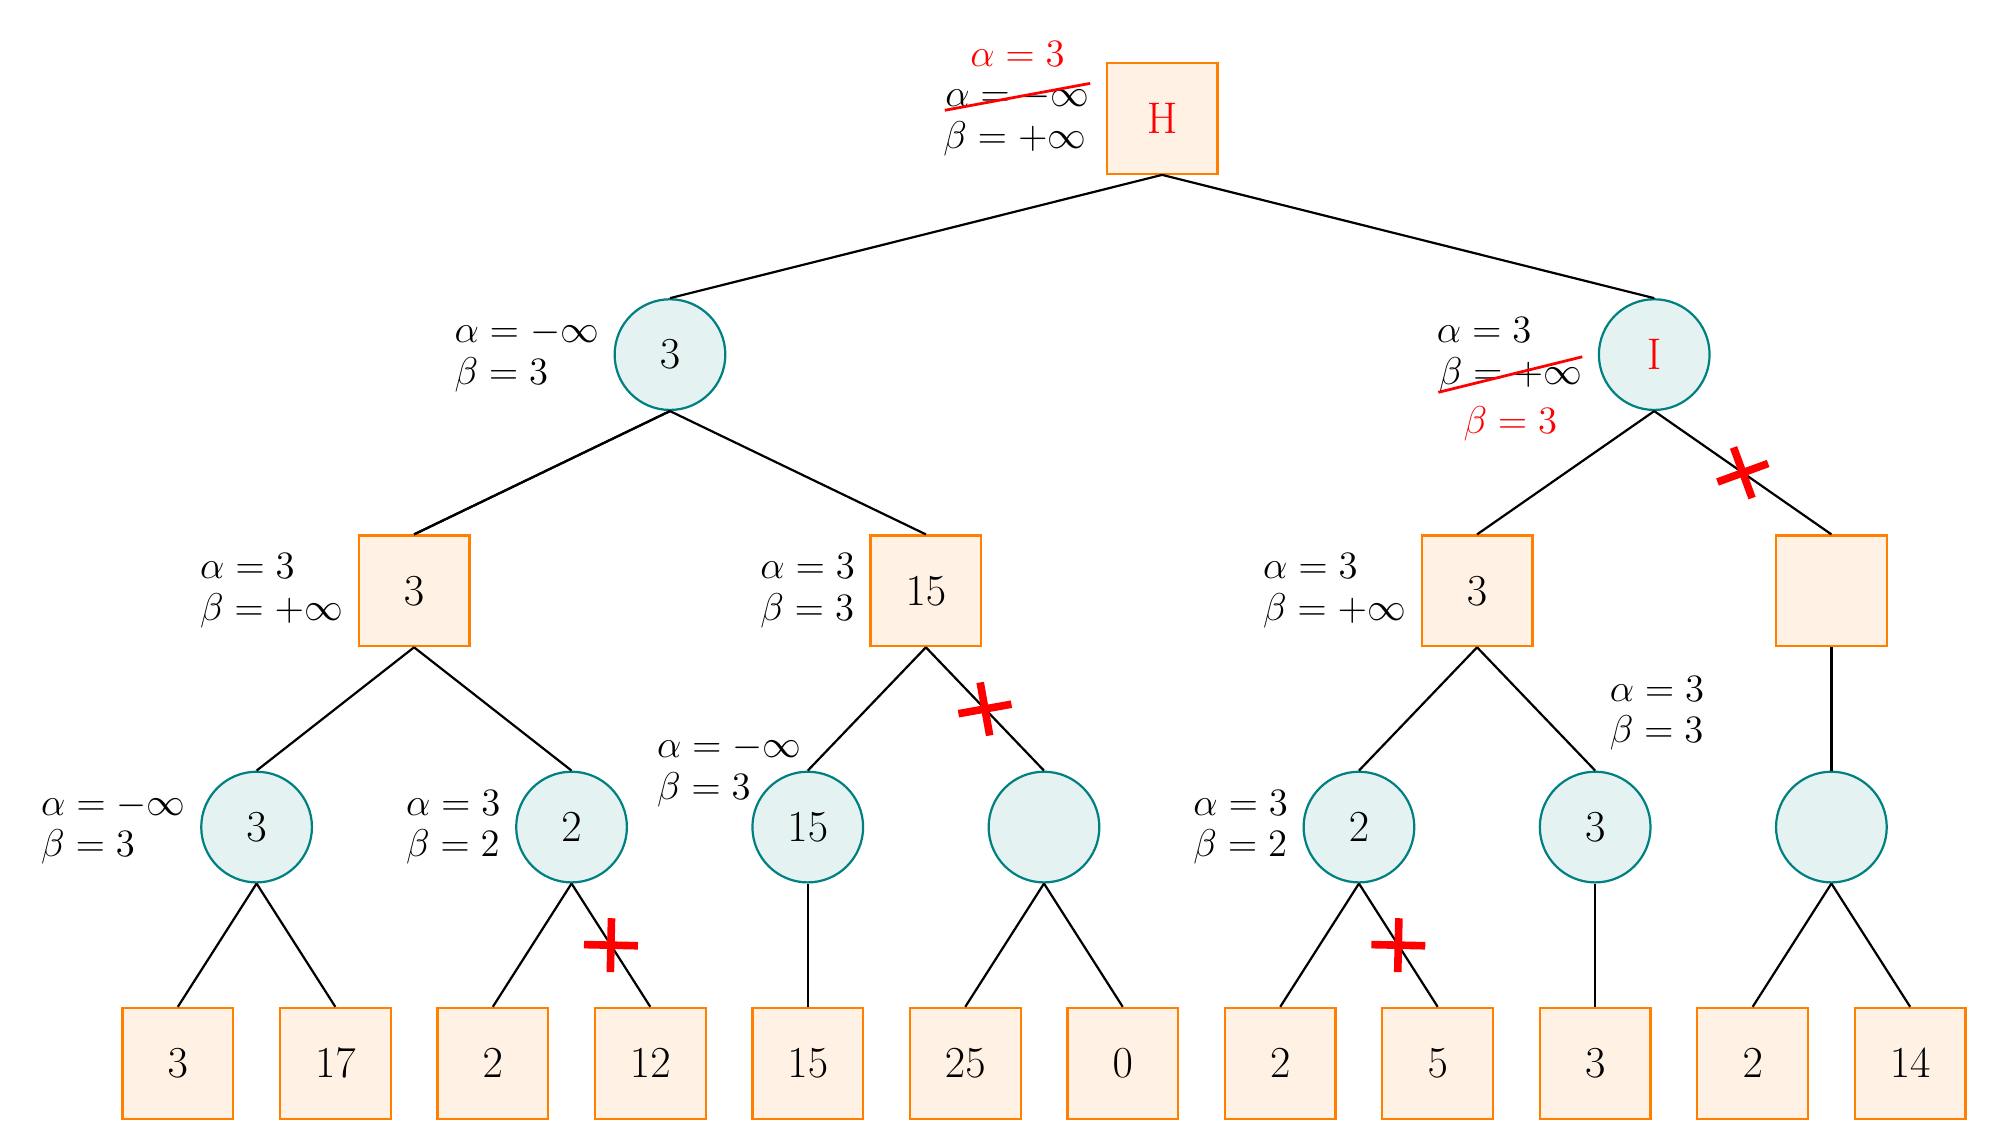
\begin{tikzpicture}[
    xscale=2, yscale=3, thick,
    max node/.style={draw,orange,rectangle,fill=orange!10!white,inner sep=-10pt,minimum size=40pt,text=black},
    min node/.style={draw,teal,circle,fill=teal!10!white,inner sep=-10pt,minimum size=40pt,text=black},
]

\node[max node] (a1)  at (0,0)  { $3$ };
\node[max node] (a2)  at (1,0)  { $17$ };
\node[max node] (a3)  at (2,0)  { $2$ };
\node[max node] (a4)  at (3,0)  { $12$ };
\node[max node] (a5)  at (4,0)  { $15$ };
\node[max node] (a6)  at (5,0)  { $25$ };
\node[max node] (a7)  at (6,0)  { $0$ };
\node[max node] (a8)  at (7,0)  { $2$ };
\node[max node] (a9)  at (8,0)  { $5$ };
\node[max node] (a10) at (9,0)  { $3$ };
\node[max node] (a11) at (10,0) { $2$ };
\node[max node] (a12) at (11,0) { $14$ };

\node[min node] (b1) at (0.5,1) { $3$ };
\node[min node] (b2) at (2.5,1) { $2$ };
\node[min node] (b3) at (4,1)   { $15$ };
\node[min node] (b4) at (5.5,1) { };
\node[min node] (b5) at (7.5,1) { $2$ };
\node[min node] (b6) at (9,1) { $3$ };
\node[min node] (b7) at (10.5,1) {};

\node[max node] (c1) at (1.5,2) { $3$ };
\node[max node] (c2) at (4.75,2) { $15$ };
\node[max node] (c3) at (8.25,2) { $3$ };
\node[max node] (c4) at (10.5,2) {};

\node[min node] (d1) at (3.125,3) { $3$ };
\node[min node] (d2) at (9.375,3) { \color{red} I };

\node[max node] (e1) at (6.25,4) { \color{red} H };

\draw (e1.south) -- (d1.north);
\draw (e1.south) -- (d2.north);
\draw (d1.south) -- (c1.north);
\draw (d1.south) -- (c2.north);
\draw (d2.south) -- (c3.north);
\draw (d2.south) -- (c4.north) node[pos=0.5,sloped] {\Cross};
\draw (d1.south) -- (c1.north);
\draw (c1.south) -- (b1.north);
\draw (c1.south) -- (b2.north);
\draw (c2.south) -- (b3.north);
\draw (c2.south) -- (b4.north) node[pos=0.5,sloped] {\Cross};
\draw (c3.south) -- (b5.north);
\draw (c3.south) -- (b6.north);
\draw (c4.south) -- (b7.north);
\draw (b1.south) -- (a1.north);
\draw (b1.south) -- (a2.north);
\draw (b2.south) -- (a3.north);
\draw (b2.south) -- (a4.north) node[pos=0.5,sloped] {\Cross};
\draw (b3.south) -- (a5.north);
\draw (b4.south) -- (a6.north);
\draw (b4.south) -- (a7.north);
\draw (b5.south) -- (a8.north);
\draw (b5.south) -- (a9.north) node[pos=0.5,sloped] {\Cross};
\draw (b6.south) -- (a10.north);
\draw (b7.south) -- (a11.north);
\draw (b7.south) -- (a12.north);

\node[left=0cm of e1.west] (active1) {\small $\begin{aligned}&\redcancel{\alpha=-\infty}\\[-4pt]&\beta=+\infty\end{aligned}$};
\node[left=0cm of d1.west] {\small $\begin{aligned}&\alpha=-\infty\\[-4pt]&\beta=3\end{aligned}$};
\node[left=0cm of d2.west] (active2) {\small $\begin{aligned}&\alpha=3\\[-4pt]&\redcancel{\beta=+\infty}\end{aligned}$};
\node[left=0cm of c1.west] {\small $\begin{aligned}&\alpha=3\\[-4pt]&\beta=+\infty\end{aligned}$};
\node[left=0cm of c2.west] {\small $\begin{aligned}&\alpha=3\\[-4pt]&\beta=3\end{aligned}$};
\node[left=0cm of c3.west] {\small $\begin{aligned}&\alpha=3\\[-4pt]&\beta=+\infty\end{aligned}$};
\node[left=0cm of b1.west] {\small $\begin{aligned}&\alpha=-\infty\\[-4pt]&\beta=3\end{aligned}$};
\node[left=0cm of b2.west] {\small $\begin{aligned}&\alpha=3\\[-4pt]&\beta=2\end{aligned}$};
\node[left=8pt of b3.west,anchor=south] {\small $\begin{aligned}&\alpha=-\infty\\[-4pt]&\beta=3\end{aligned}$};
\node[left=0cm of b5.west] {\small $\begin{aligned}&\alpha=3\\[-4pt]&\beta=2\end{aligned}$};
\node[above=0cm of b6.north,anchor=south west] {\small $\begin{aligned}&\alpha=3\\[-4pt]&\beta=3\end{aligned}$};
\node[above=-7pt of active1.north] {\small\color{red} $\alpha=3$};
\node[below=-7pt of active2.south] {\small\color{red} $\beta=3$};

\end{tikzpicture}

\end{document}
